\chapter{SOLVING WORD PROBLEMS IN GEOMETRY}
\section*{INTRODUCTION}
This module is intended to give an overview on solving word problems in geometry. It presents
the different steps in problem solving as designed by Polya. It also contains sample word problems for
the participants to solve. Assessment questions are also given.
\section*{OBJECTIVES}
After completion of the module, the participants are expected to:
\begin{enumerate}
\item Apply the different steps in problems solving
\item Determine the appropriate strategy to use in solving a word problem.
\item Use variety of problem solving strategies in solving word problems.
\item Solve the word problems accurately.
\item Appreciate the importance of problem solving in a mathematics curriculum.
\item Gain confidence in doing problem solving
\item Create more interesting word problems.
\item Integrate or connect geometry to origami, the art of paper folding.
\end{enumerate}
\section*{DISCUSSION}
The National Council of Teachers of Mathematics (NCTM) gives the following definitions on the
nature of mathematics: mathematics is a study of patterns and relationships, it is a way of thinking, it is
an art, it is a language and it is a tool. NCTM identified five broad goals required to meet the students’
mathematical needs for the 21st century. They are as follows: students should (1) value mathematics,
(2) reason mathematically, (3) communicate mathematics, (4) solve problems and (5) develop
confidence.

Problem solving is the heart of mathematics. It is a process. It is the means by which an
individual uses previously acquired knowledge, skills and understanding to satisfy the demands of an
unfamiliar situation. Students must be exposed to a variety of problems – problems that vary in context,
in level of difficulty and in methods in solving the problem. But what is really a problem or a word
problem specifically? A word problem is a mathematical proposition that a student has never
experienced solving. What are the purposes of word problems? The following are the different
purposes of word problems: (1) to prepare the students for real life, (2) to develop children’s logical and
abstract thinking and mental discipline, and (3) to motivate students. Hence a word problem should
simulate real life situations, events, and places that students can experience firsthand. In this way the
students will be able to see the importance of mathematics in their life.

George Polya, a mathematician, devised the following \Bold{four-step method} in solving word problems:

\begin{enumerate}
\item \textbf{Read and understand the problem}\index{four-step method!Read and understand the problem}

Read and reread the problem. Ask the following questions: What is the situation all
about? What information is given? What are the different assumptions? What information is
missing? What are you being asked to find or to do? You can make a list in this format

Information given (GIVEN): \makebox[2in]{\hrulefill}

Goals of the problem (REQUIRED): \makebox[2in]{\hrulefill}

\item \textbf{Plan how to solve the problem. Try a strategy}\index{four-step method!Try a strategy}\index{four-step method!Plan how to solve the problem}

In developing a plan to solve the problem ask the following questions: Have you ever
worked a similar problem before? Will you estimate or calculate? What strategy (ies) can you
use? Consider the different strategies in solving problem that you know. The following could be
your shopping list on the different problem solving strategies: draw a diagram, make a table,
write an equation, guess and check (trial and error), look for a pattern, solve a simpler problem,
work backward. Word problems can be solved using different strategies.

\item \textbf{Solve the problem/ Carry out the plan.}\index{four-step method!solve the problem}\index{four-step method!carry out the plan}

As you implement the strategy that you choose, ask the following questions: Did you
calculate correctly? What is the solution? Did you interpret correctly? Did you answer the
question?

\item \textbf{Look back}\index{four-step method!look back}

Most students forget this last part especially if they are solving a problem set or many
problems. The most important question that should be asked here is: “Is the calculated answer
reasonable?”
\end{enumerate}
However there is also a danger in over-using Polya's four steps in problem solving. Students
may think that problem solving is one directional that follows the given steps above as if it's the
prescribed recipe. Emphasize to students that with challenging problems, the actual problem solving
becomes a process whereby the solver keeps a mental "check" of the progress, and corrects himself if
progress is not made. He may go one route, notice it won't work, go backwards a bit, and then, take
another route. In other words, devising plans and carrying them out can occur somewhat
simultaneously, and we can go back and forth. Lastly, not all problems can be solved using the steps
above.

\subsection*{Problems Involving Perimeters}
\begin{example}
\Item The perimeter of a square is 28 cm. Find the length of each side.

\Solution

\textit{Geometry Concept:} A square is a quadrilateral (4-sided polygon) with four congruent sides. Its four
interior angles are all right angles. The formula for the perimeter ($P$) of a square is $P = 4s$ and its area ($A$) is $A = s^2$ where $s$ is the side of the square.

\begin{tikzpicture}
\draw (0,0) -- (1,0) -- (1,1) -- (0,1) -- cycle;
\node [below] at (0.5,0) {$s$};
\node [right] at (1,0.5) {$s$};
\node [above] at (0.5,1) {$s$};
\node [left] at (0,0.5) {$s$};
\end{tikzpicture}
\begin{align*}
P&=4s\\
28&=4s\\
\therefore s&=7
\end{align*}
Therefore, the square has side of length 7 cm.
\end{example}

\begin{example}
\item The length of a rectangular garden is 3 meters more than its width. If the perimeter of the garden is
50 meters, what is the area of the rectangle?

\Solution

\textit{Geometry Concept}

A rectangle is a quadrilateral (4-sided polygon) with two pairs of congruent
and parallel sides. Its four interior angles are all right angles.
The formula for the perimeter ($P$) of a rectangle is $P = 2L + 2W$ where $L$ is
the length and $W$ is the width of the rectangle.

\begin{tikzpicture}[xscale=2]
\draw (0,0) -- (1,0) -- (1,1) -- (0,1) -- cycle;
\node [below] at (0.5,0) {$L$};
\node [right] at (1,0.5) {$W$};
\node [above] at (0.5,1) {$L$};
\node [left] at (0,0.5) {$W$};
\end{tikzpicture}

\textit{Representation}
\begin{align*}
W&=\text{width of the rectangle}\\
L&=W+3
\end{align*}

\textit{Equation:}
\begin{align*}
50 &= 2(W + 3) + 2W && \text{Using the formula for perimeter.}\\
50 &= 2W + 6 + 2W \\
44 &= 4W \\
W &= 11 \\
L &= 11 + 3 = 14 \\
A &= (14)(11) = 154 && \text{Using the formula for area.}
\end{align*}

Therefore, the rectangle has an area of 154 $\cm^2$.
\end{example}

\begin{example}
\Item The longest side of a triangle is twice as long as the shortest side and is also 2 cm longer than the third side. If the perimeter of the triangle is 33 cm, what is the length of each side?

\Solution

\textit{Geometry Concept:}

A triangle is a 3-sided polygon. The formula for the perimeter ($P$) of a triangle is
$P = a + b + c$ where $a$, $b$ and $c$ are the sides of the triangle.

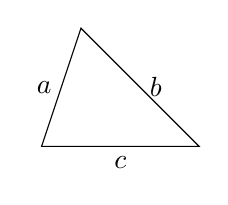
\begin{tikzpicture}
\draw (0,0) -- (2,0) -- (0.5,1.5) -- cycle;
\node [below] at (1,0) {$c$};
\node [right] at (1.25,0.75) {$b$};
\node [left] at (0.25,0.75) {$a$};
\end{tikzpicture}

\textit{Representation}

\begin{align*}
a&=x && \text{shortest side of the triangle}\\
b&=2x && \text{longest side}\\
c&=2x-2 && \text{third side}
\end{align*}

\textit{Equation}

\begin{align*}
33 &= x + 2x + 2x - 2 && \text{(Using the formula for the perimeter.)}\\
35 &= 5x\\
x &=7\\
a&=x=7\\
b&= 2x = 14\\
c &= 2x - 2 = 12
\end{align*}
Therefore, the sides of the triangle are 7 cm, 12 cm and 14 cm.
\end{example}

\begin{example}
\Item What is the measure of the base of an isosceles triangle if its perimeter is 50 cm and the length of one of its congruent sides exceeds the length of the base by 10 cm?

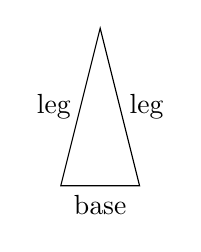
\begin{tikzpicture}[yscale=2]
\draw (0,0) -- (1,0) -- (0.5,1) -- cycle;
\node [below] at (0.5,0) {base};
\node [right] at (0.75,0.5) {leg};
\node [left] at (0.25,0.5) {leg};
\end{tikzpicture}

\Solution

\textit{Geometry Concept}

An isosceles triangle is a triangle with two congruent sides. The congruent sides are
called legs while the non-congruent side is called the base.

\textit{Representation}

\begin{align*}
x&=\text{length of the base of the triangle}\\
  x+10&=\text{length of the leg of the triangle}
\end{align*}

\textit{Equation}

\begin{align*}
50 &= x + 2(x + 10) && \text{(Using the formula for perimeter of triangles.)}\\
50 &= x + 2x + 20\\
30 &= 3x\\
x &= 10
\end{align*}
Therefore, the base of the isosceles triangle is 10 cm.
\end{example}

\subsection*{PROBLEMS INVOLVING ANGLES OF POLYGONS}
\begin{example}
\Item The first angle of a triangle is triple that of the smallest angle. The second angle is 5 degrees more than the first angle. What is the measure of the smallest angle?

\Solution

\textit{Geometry Concept}

A triangle has three interior angles and their measures sum up to 180 degrees.

\textit{Representation}
\begin{align*}
x &= \text{smallest angle of the triangle}\\
3x &= \text{first angle of the triangle}\\
3x + 5 &= \text{second angle of the triangle}
\end{align*}
\textit{Equation}
\begin{align*}
x + 3x + 3x + 5 &= 180 && \text{(Sum of the angles of a triangle is $180^{\circ}$.)}\\
7x &= 175\\
x &= 25
\end{align*}
Therefore, the measure of the smallest angle of the triangle is 25 degrees.
\end{example}
